\section{Verification stages and release-rule calibration}
\label{S-sec:s-verification}

\begin{table*}[t]
\caption{Candidate recovery and conversion on all 1781 3DLoMatch+FPFH pairs. Native, winner-only ICP, finishing and release are recall (\%); $C$ is correct-pose coverage after the fixed finishing procedure. The gap $C-\mathrm{Native}$ is in percentage points, computed before rounding; $E$ is the percentage of covered pairs successfully released. Coverage uses ground truth only for diagnosis.}
\label{S-tab:s-utilization}
\centering
\small
\begin{tabular}{lrrrrrrr}
\toprule
Frontend & Native & Winner ICP & Finishing & Release & Coverage $C$ & $C-\mathrm{Native}$ & $E$ \\
\midrule
RANSAC-1M & 35.1 & 39.9 & 45.7 & 48.8 & 54.2 & 19.1 & 90.1 \\
SC$^2$-PCR & 39.0 & 42.2 & 49.7 & 52.6 & 59.8 & 20.8 & 87.9 \\
MAC & 40.0 & 43.2 & 49.4 & 51.6 & 59.7 & 19.8 & 86.4 \\
TurboReg & 38.5 & 41.8 & 49.0 & 51.5 & 56.4 & 18.0 & 91.3 \\
NGR & 40.3 & 42.8 & 48.7 & 51.1 & 56.4 & 16.1 & 90.6 \\
NGRR-LS & 40.4 & 43.0 & 49.6 & 53.1 & 59.2 & 18.8 & 89.8 \\
\bottomrule
\end{tabular}

\end{table*}

The native-to-refined-pool gap is 16.1--20.8 percentage points for each of the six frontends (\cref{S-tab:s-utilization}). Coverage measures the pool after prescribed allocation and refinement; those hypotheses need not have been correct in their coarse form. Backend timings are measured separately on a 100-pair subset at the specified CPU thread count.

\begin{figure*}[t]
\centering
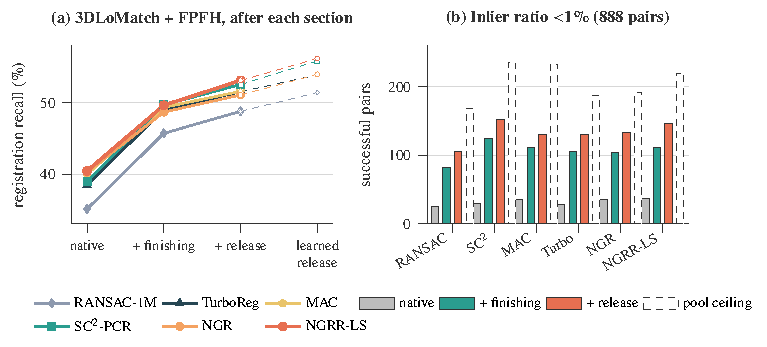
\includegraphics[width=.86\linewidth]{shared/figures/fig_results.pdf}
\caption[Recall after each section and on pairs below 1\% inliers]{(a) Recall on 3DLoMatch+FPFH after each section, for every frontend; dashed: the optional learned assay. (b) Pairs with an input inlier ratio below 1\% (888 of 1781): successes of the native output, after finishing, after the release assay, and the refined-pool ceiling. Panel (b) also appears as \main{\cref*{fig:dilute}}(a).}
\label{S-fig:s-results}
\end{figure*}

\paragraph{Recall after each stage.} \Cref{S-fig:s-results}a follows every frontend on 3DLoMatch+FPFH through finishing and release. Training-free verification raises recall by 10.8--13.7 percentage points for all six frontends, and the optional learned assay adds another 1.8--3.3 percentage points on 3DLoMatch with FPFH and FCGF. \Cref{S-fig:s-results}b isolates the 888 pairs with an inlier ratio below 1\%. The native frontends register 26--37 of them. Finishing raises this to 82--124, and the release assay to 106--152, 3.7--5.1 times the native count; the learned assay reaches 148--193 (not run for MAC). With the same verification SC$^2$-PCR releases the most of these pairs (152) and \ls{} 147.

\paragraph{Coverage and recall, unit by unit.} \main{\cref*{tab:joint}} reports stage gains and refined-pool conversion; \main{\cref*{tab:units}} isolates the generation controls. Coverage is the share of pairs whose refined pool, containing up to 32 candidates, includes a correct pose. Fixing the frontend and finishing procedure fixes this coverage; release selects within the resulting pool. Site capacity mainly changes coverage: on 3DLoMatch it adds 2.8 and 1.9 points of coverage with FPFH and FCGF (50 and 33 pairs), but changes the native output by only 0.1 and 0.2 points, and by at most 0.5 on any cohort. Finishing and release increase recall within that coverage: finishing adds 9.2 and 3.8 points and the release assay another 3.5 and 3.7, and the full verification procedure converts 89.8\% and 92.7\% of the coverage into registrations, close to the rate it achieves for \ngr{} (90.6\% and 93.7\%). The capacity's final gain on 3DLoMatch+FPFH (2.0 points, 36 pairs) thus comes from its coverage gain (50 pairs) processed by verification that converts both frontends' coverage at about the same rate; it reflects better candidate generation despite little change in the native output.

\paragraph{Finishing controls.} Refining only the native winner gives 43.0\% instead of 49.6\% (\ls, 3DLoMatch+FPFH). Refining the top 32 hypotheses with the same ICP and keeping the largest truncated correspondence support gives 32--72 fewer registered pairs than the finishing step for each of RANSAC, SC$^2$-PCR, MAC, TurboReg and \ngr{}; selecting by the highest Open3D fitness gives still lower recall (25.3--38.4\%).

\paragraph{Single-channel controls.} Over the nine cohorts, releasing by support alone or by residual shape alone gives 9760 and 9759 registered pairs with \ls{}, against 9920 for their minimum, and for every frontend the minimum releases more pairs than either channel alone.

\begin{table*}[t]
\caption[Release rules on the same refined pools]{Release rules on the same refined pools, limited to the first 32 candidates. Training: 12\,000 cells (3000 pairs, four frontends); test: 72\,117 cells (nine cohorts, every frontend where it completed; MAC's 3497 failed pairs are excluded). A cell succeeds if its selected candidate is correct. $s$, $h$: the normalized channels of the release assay (\main{\cref*{eq:assay}}, also in the first row); ties by $s$, $h$, queue order (lexicographic $s$-then-$h$ is equivalent to the $s$-only rule). Against \main{\cref*{eq:assay}}: test cells released by the rule but not by it and vice versa, and test pairs on which the rule releases more or fewer of the frontends' cells; the cells of one pair share its scans and correspondences, so $p$ is from a sign test over pairs, Holm-corrected over the seven rules. Bottom: the expected count of a uniform choice inside the non-dominated set, and bounds that no rule on these pools can exceed (the non-dominated set bounds every rule above).}
\label{S-tab:s-rules}
\centering\footnotesize
\begingroup
\let\origcref\cref
\renewcommand{\cref}[1]{\origcref{#1}}
\begin{tabular}{lrrrrr}
\toprule
Release rule & Training $\uparrow$ & Test $\uparrow$ & Cells & Pairs & Holm $p$ \\
\midrule
$\min(s,h)$ & 9209 & 58922 &  &  &  \\
support $s$ only & 8925 & 58020 & $+172/-1074$ & $+81/-399$ & $1\times10^{-50}$ \\
shape $h$ only & 8900 & 57812 & $+1021/-2131$ & $+362/-779$ & $6\times10^{-35}$ \\
$\lambda s+(1-\lambda)h$, $\lambda=0.3$ from training & \textbf{9290} & \textbf{59288} & $+624/-258$ & $+258/-112$ & $9\times10^{-14}$ \\
product $sh$ & 9208 & 58960 & $+140/-102$ & $+84/-62$ & 0.16 \\
harmonic mean & 9211 & 58964 & $+135/-93$ & $+81/-55$ & 0.10 \\
rank sum (Borda) & 9164 & 58806 & $+371/-487$ & $+190/-224$ & 0.16 \\
\midrule
uniform choice in the non-dominated set (expected) & & 58075 & & & \\
non-dominated set contains a correct pose & & 60311 & & & \\
pool contains a correct pose (ceiling) & 9754 & 61144 & & & \\
\bottomrule
\end{tabular}

\endgroup

\end{table*}

\subsection{Null calibration and alternative release rules}

The minimax-regret argument of \main{\cref*{sec:assay}} covers linear trade-offs between two normalized surrogates, not registration success, and the shape channel rests on a null that real scans need not satisfy. We test both on the stored refined pools of every frontend and cohort, with no new generation or refinement (\cref{S-tab:s-rules}). A cell is one frontend on one test pair. These comparisons were added after the main evaluation; each was pre-registered before it was run, and none changes the reported pipeline.

\paragraph{Null model and ranking.} For clearly wrong candidates (RE${}>30^\circ$ or TE above three times the success threshold) the null predicts $\bar u\approx\frac12$. We measure medians of 0.17--0.24 on the indoor cohorts and 0.28--0.33 on KITTI and ETH, and $\bar u<\frac12$ for at least 99.7\% of the wrong candidates in every cohort: wrong poses can also align planar patches, producing concentrated residuals. $\psi$ is therefore not a calibrated likelihood ratio. Correct candidates nevertheless have lower residual means (medians 0.12--0.18), and in pools containing both correct and incorrect candidates, the shape channel separates them with a pool-averaged AUC of 0.83--0.99, the support channel with 0.89--1.00, and their minimum with 0.89--1.00.

\paragraph{Alternative release rules.} The product and the harmonic mean of the two channels, also parameter-free, succeed on 38 and 42 more of the 72\,117 test cells than the release assay (0.05--0.06\%). These differences are not significant when tested over pairs (better on 84 and 81 pairs, worse on 62 and 55; Holm $p=0.16$ and $0.10$). Support alone and shape alone succeed on 902 and 1110 fewer cells, and a rank sum succeeds on 116 fewer (not significant by pair). A weighted sum whose one weight is chosen on the training cohort ($\lambda=0.3$) releases 366 more ($+624/-258$ cells; better on 258 pairs and worse on 112, Holm $p=9\times10^{-14}$), gains in eight of the nine cohorts (one tie), and raises \ls{} from 9920 to 9992 registered pairs over the nine cohorts. Learning the release from 26 features raises it to 10\,084. The minimax guarantee concerns surrogate trade-offs. For registration, two other parameter-free combinations perform similarly, one fitted weight improves success on about 0.5\% of cells, and the learned assay improves it further. We keep \main{\cref*{eq:assay}}, frozen before these comparisons, as the training-free default. Every rule here chooses inside the non-dominated set of the pool, which holds a correct candidate in 60\,311 of the 61\,144 cells whose pool does. A uniform choice inside it would release 58\,075.

\subsection{Allocation against plain Top-K at matched refinement budget}
\label{S-sec:s-topk}

This control was pre-registered before it was run and does not change the reported pipeline. Each cell is one frontend on one test pair. A is finishing's published allocated pool, with $n_i$ actual ICP calls. B is plain Top-K with exactly the same $n_i$ calls: it begins with the native winner, then takes the correspondence-support-ranked shortlist after the same $5^\circ$/$\tau$ suppression. When that shortlist is shorter than $n_i$, B fills the remaining calls with the next legal raw hypotheses in the same order. C refines the complete stored Top-K bank, up to 32 candidates. All three arms use the same SurfaceICP implementation and the same release rule of \main{\cref*{eq:assay}}. The support and shape channels use the same query points. Ground truth is read only after the final candidate has been selected.

The reproducibility checks all pass. A reproduces the published release in every cell. Recomputing A on the B/C evidence path reproduces its information scores to within $1.1\times10^{-15}$ and its residual moments exactly. The A and C coverage values match the stored records, every recomputed shortlist has the expected length, and the run contains no frontend errors.

Across nine test cohorts, A and B each make 1\,216\,817 ICP calls. A releases 58\,922 correct cells and B releases 58\,340, a paired difference of $+849/{-}267$ (\cref{S-tab:s-topk}; MAC's cells hold the pools of our earlier Python adaptation, and without them the main paper reports 51\,900 against 52\,372, $+693/{-}221$). Six correspondence frontends remain significant after Holm correction, with the largest adjusted $p$ value $8.9\times10^{-7}$. LGR has no significant difference ($+10/{-}7$, $p=0.63$). Cells from the same pair are not independent, so we also aggregate the A--B difference per point-cloud pair. A is better on 401 pairs and B on 150 ($p=2.1\times10^{-27}$). After grouping descriptor variants of the same scan pair, the result is 368 scan pairs versus 137 ($p=1.9\times10^{-25}$).

The mechanism is visible in the coverage and selection decomposition. A's refined pools contain a correct pose in 61\,144 cells, compared with 59\,784 for B, a gain of 1\,360 cells. The final gain is smaller because the fixed release rule selects 58\,922 of A's covered cells (96.37\%) and 58\,340 of B's covered cells (97.59\%). Allocation therefore improves candidate recovery. It does not raise conditional selection effectiveness under the fixed release rule. On 3DLoMatch+FPFH with \ls{}, A, B and C register 946, 907 and 908 of 1781 pairs, corresponding to 53.12\%, 50.93\% and 50.98\%.

C makes 1\,747\,401 ICP calls, 43.6\% more than A, and releases 58\,514 correct cells. This shows that the A--B difference is not explained by using more refined candidates. The control matches the number of ICP calls, not total wall-clock time. On the 100-pair 3DLoMatch+FPFH timing subset, the frozen implementation takes 2.45\,s per pair for A and 0.87\,s for B with SC$^2$-PCR. For TurboReg, the corresponding medians are 6.20\,s and 1.49\,s. The extra time comes from scoring candidates before ICP. The compiled finishing implementation used in the main timing table takes 0.09--0.11\,s per pair; a compiled B implementation was not measured.

\begin{table*}[t]
\centering
\footnotesize\setlength{\tabcolsep}{3pt}%
\begin{tabular}{lrrrrrrrr}
\toprule
& & \multicolumn{3}{c}{Released correct} & \multicolumn{2}{c}{A vs.\ B} & \multicolumn{2}{c}{ICP calls} \\
\cmidrule(lr){3-5}\cmidrule(lr){6-7}\cmidrule(lr){8-9}
Frontend & Cells & A & B & C & $+a/{-}b$ & Holm $p$ & A $=$ B & C \\
\midrule
RANSAC-1M & 12035 & 9771 & 9701 & 9729 & $+111/{-}41$ & $4\times10^{-8}$ & 179562 & 252148 \\
SC$^2$-PCR & 12035 & 9948 & 9885 & 9902 & $+109/{-}46$ & $9\times10^{-7}$ & 244190 & 367848 \\
MAC & 8538 & 6550 & 6440 & 6481 & $+156/{-}46$ & $2\times10^{-14}$ & 188278 & 273216 \\
TurboReg & 12035 & 9886 & 9746 & 9783 & $+186/{-}46$ & $3\times10^{-20}$ & 255238 & 385120 \\
LGR (GeoTr) & 3404 & 2990 & 2987 & 2990 & $+10/{-}7$ & 0.63 & 69221 & 108928 \\
NGR & 12035 & 9857 & 9753 & 9786 & $+140/{-}36$ & $7\times10^{-15}$ & 128805 & 158991 \\
\ls{} & 12035 & 9920 & 9828 & 9843 & $+137/{-}45$ & $2\times10^{-11}$ & 151523 & 201150 \\
\midrule
All & 72117 & 58922 & 58340 & 58514 & $+849/{-}267$ & -- & 1216817 & 1747401 \\
\bottomrule
\end{tabular}%

\caption{Allocation against plain Top-K over the nine test cohorts. A is finishing's allocated pool and reproduces the published release. B is plain Top-K with A's actual ICP calls on every cell. C is the full stored Top-K bank. All arms use the same ICP and release rule. $+a/{-}b$ gives cells registered by A but not B, and vice versa. The $p$ values are exact McNemar tests with Holm correction over the seven frontends. MAC: the pools of our earlier Python adaptation, only pairs within its resource limit (\cref{S-sec:s-maccpp}).}
\label{S-tab:s-topk}
\end{table*}

\subsection{Standard and published verification rules on the same pools}
\label{S-sec:s-selectors}

The comparison of the eight external rules was pre-registered before it was run; FS-TCD was added afterwards. Neither changes the reported pipeline. Every rule chooses one candidate inside the same refined pool as the release, so generation, allocation and ICP are identical; no ICP is re-run. A cell is one frontend on one test pair, as in \cref{S-tab:s-rules}; MAC's cells hold the stored pools of our earlier Python adaptation (\cref{S-sec:s-maccpp}). The main paper reports these comparisons without MAC's cells: release registers 52\,372 of 63\,579 cells, CorAl 51\,432 and prerejective 51\,376; matched Top-K 51\,900 ($+693/{-}221$) and full Top-32 52\,033 with 43.3\% more ICP calls; release 31\,064 against FS-TCD 29\,891 of 39\,590 cells ($+1654/{-}481$). Pool A is the finishing step's refined pool (its first 32 valid candidates). Pool C is the complete plain Top-K bank of \cref{S-sec:s-topk}.

\paragraph{Rules.} Five scores come from the finishing quantities or ICP: $M\sqrt G$, $M$, $G$, Open3D fitness with RMSE as tie-break, and a truncated Chamfer distance. Eight external training-free rules are our implementations of published verification scores on the voxelized observed clouds. LCP counts source points within $\delta$ of the target~\cite{aiger2008fpcs}, and OpenGR's weighted LCP~\cite{mellado2014super4pcs} weights them by a bisquare kernel. PCL's greedy verification~\cite{rusu2011pcl} subtracts $\lambda$ times the unexplained source points from the explained target points. The single-hypothesis GHV cost~\cite{aldoma2012ghv}, without occlusion reasoning, rewards normal-consistent explained points and penalizes outliers and clutter. SAC-IA~\cite{rusu2009fpfh} minimizes the truncated sum of distances. The prerejective score~\cite{buch2013prerejective} takes the smallest inlier mean squared distance among candidates whose inlier share is at least $g$. CorAl~\cite{adolfsson2021coral} minimizes the joint minus separate differential entropy of radius-$r$ neighborhoods, and MPV~\cite{razlaw2015mpv} minimizes the mean plane variance of the joint neighborhoods. Distances and radii are in units of $\tau$, and neighborhoods are exact. Each rule except SAC-IA has one parameter, chosen on the training cohort's pool A from a registered grid: $\delta=0.5$ for LCP and WLCP, $\lambda=0.5$, a GHV weight of 0.5, $g=0.1$, $r=3$ for CorAl and $r=2$ for MPV. With library-style defaults, prerejective registers 57\,780 cells and CorAl 56\,678. GT labels the chosen candidates only after every rule has chosen.

\paragraph{Results.} \Cref{S-tab:s-selector-full} lists every rule and \cref{S-tab:s-selector-cohort} the cohorts. Release registers 58\,922 cells on pool A and 58\,514 on pool C. The best external rules are CorAl with 57\,792 on pool A and prerejective with 56\,851 on pool C; with its default parameter, prerejective reaches 57\,780 on pool A. Every comparison favors release at the cell level (McNemar with Holm, $p\le9.8\times10^{-73}$, the largest for CorAl), over pairs and over scan pairs. Over pairs and scan pairs the weakest is prerejective, with 830 against 386 pairs ($p=8.5\times10^{-38}$) and 635 against 306 scan pairs ($p=3.3\times10^{-27}$). Overlap scores fail where overlap is low: on 3DLoMatch+FPFH, ICP fitness releases 2494 of 10\,686 cells, fewer than the frontends' native outputs. Against the best external rule of each cohort, the lead sums to 433 cells, two thirds of it on 3DLoMatch+FPFH. It is 287 cells on 3DLoMatch+FPFH and 81 on 3DMatch+FPFH, but at most 5 cells with FCGF on 3DMatch and 3DLoMatch, and 27 and 65 with GeoTransformer. On the saturated ETH and KITTI+FCGF cohorts, surface-overlap rules reach or nearly reach the ceiling (4175 and 2852 of 2854 cells), and release is within 28 and 6 cells. None of these rules reaches the 58\,075 cells of a uniform choice inside the non-dominated set of \cref{S-sec:s-verification}. The Python implementation of all eight external rules together takes a median of 170\,s per pair with exact neighborhoods. This is the cost of the experiment, not a speed comparison.

\paragraph{FS-TCD of SC$^2$-PCR++.} SC$^2$-PCR++~\cite{chen2023sc2pp} selects its model with a feature- and spatial-consistency constrained truncated Chamfer distance (FS-TCD). We port its \texttt{select\_best\_trans} and \texttt{post\_refinement} line by line from the official code (commit 5a654fd) to the CPU and apply it to the same pool A. The one-to-one matches are the cached correspondences, and the relaxed matches are each source point's 100 nearest target keypoints in descriptor space, as in the official matcher. The settings are those the official test scripts execute: inlier threshold 0.1\,m and FS-TCD threshold 0.05\,m indoors, 0.6\,m and 0.05\,m on KITTI. The rule needs keypoint descriptors, so it is evaluated on the six cohorts with descriptor archives. The cells are those of pool A above, and the recomputed release matches the published release in every cell. Unlike the official loaders, we use all cached keypoints without random subsampling. The KITTI configuration file lists an FS-TCD threshold of 0.1\,m, which gives 35\,133 cells in total. Release registers more cells in every cohort (\cref{S-tab:s-fstcd}), 36\,495 against 35\,102 of 46\,710 ($+1991/{-}598$, exact McNemar $p<10^{-170}$). Scoring each chosen candidate after its post-refinement, or never overwriting the one-to-one matches, gives 35\,210 and 35\,119 cells.

\begin{table}[t]
\caption{All selection rules on pool A, with pool C's count (\cref{S-sec:s-selectors}). Correct cells over the nine test cohorts. Pairs $+/{-}$: pairs on which release registers more or fewer of the frontends' cells than the rule.}
\label{S-tab:s-selector-full}
\centering
\footnotesize\setlength{\tabcolsep}{2.5pt}%
\begin{tabular}{@{}lrrrrr@{}}
\toprule
Rule on pool A & All & 3DLoMatch & Others & Pairs $+/{-}$ & Pool C \\
Cells & 72117 & 32674 & 39443 & & 72117 \\
\midrule
Release (ours) & 58922 & 21491 & 37431 & -- & 58514 \\
\midrule
$M\sqrt{G}$ & 57696 & 20575 & 37121 & $484/62$ & -- \\
$M$ & 56997 & 20405 & 36592 & $679/78$ & -- \\
$G$ & 51913 & 15370 & 36543 & $2064/237$ & -- \\
Truncated Chamfer & 51902 & 15330 & 36572 & $2076/242$ & -- \\
Fitness + RMSE & 49355 & 13621 & 35734 & $2801/190$ & -- \\
\midrule
CorAl~\cite{adolfsson2021coral} & 57792 & 21088 & 36704 & $1066/488$ & 55245 \\
Prerejective~\cite{buch2013prerejective} & 57704 & 20661 & 37043 & $830/386$ & 56851 \\
MPV~\cite{razlaw2015mpv} & 57287 & 21100 & 36187 & $1179/464$ & 54733 \\
GHV~\cite{aldoma2012ghv} & 54582 & 17661 & 36921 & $1503/284$ & 55711 \\
WLCP~\cite{mellado2014super4pcs} & 53848 & 16869 & 36979 & $1601/279$ & 55567 \\
LCP~\cite{aiger2008fpcs} & 52644 & 15916 & 36728 & $1875/245$ & 54883 \\
SAC-IA~\cite{rusu2009fpfh} & 51898 & 15327 & 36571 & $2070/231$ & 54398 \\
Greedy~\cite{rusu2011pcl} & 49441 & 13669 & 35772 & $2782/206$ & 52574 \\
\midrule
Ceiling & 61144 & 23106 & 38038 & & 60336 \\
\bottomrule
\end{tabular}%

\end{table}

\begin{table*}[t]
\caption{Selection rules on pool A by cohort (correct cells, all frontends). Bold: the most correct cells in the row, excluding the ceiling. Fitness and $M\sqrt G$ are from the finishing records, the other rules as in \cref{S-tab:s-selector-full}.}
\label{S-tab:s-selector-cohort}
\centering
\footnotesize\setlength{\tabcolsep}{3pt}%
\begin{tabular}{@{}lrrrrrrrrr@{}}
\toprule
Cohort & Cells & Release & $M\sqrt G$ & Fitness & CorAl & Prerej. & MPV & GHV & Ceiling \\
\midrule
3DM FPFH & 9719 & \textbf{8794} & 8635 & 7869 & 8651 & 8713 & 8539 & 8622 & 9149 \\
3DM FCGF & 9428 & \textbf{8918} & 8871 & 8264 & 8913 & 8880 & 8911 & 8619 & 9065 \\
3DM GeoTr & 9822 & \textbf{9402} & 9394 & 9259 & 9367 & 9359 & 9375 & 9329 & 9468 \\
3DLo FPFH & 10686 & \textbf{5511} & 5108 & 2494 & 5224 & 5178 & 5187 & 4199 & 6166 \\
3DLo FCGF & 10681 & \textbf{7102} & 6667 & 3813 & 7089 & 6832 & 7100 & 5357 & 7677 \\
3DLo GeoTr & 11307 & \textbf{8878} & 8800 & 7314 & 8775 & 8651 & 8813 & 8105 & 9263 \\
ETH FPFH & 4278 & 4147 & 4056 & 4166 & 3707 & 3915 & 3291 & \textbf{4175} & 4175 \\
KITTI FPFH & 3330 & \textbf{3324} & \textbf{3324} & \textbf{3324} & 3220 & \textbf{3324} & 3223 & \textbf{3324} & 3327 \\
KITTI FCGF & 2866 & 2846 & 2841 & \textbf{2852} & 2846 & \textbf{2852} & 2848 & \textbf{2852} & 2854 \\
\bottomrule
\end{tabular}%

\end{table*}

\begin{table}[t]
\caption{SC$^2$-PCR++'s FS-TCD selection against release on pool A of the six cohorts with descriptors (correct cells, all frontends). $+/{-}$: cells registered by release only and by FS-TCD only.}
\label{S-tab:s-fstcd}
\centering
\footnotesize\setlength{\tabcolsep}{3pt}%
\begin{tabular}{@{}lrrrrr@{}}
\toprule
Cohort & Cells & Release & FS-TCD & $+/{-}$ & Ceiling \\
\midrule
3DMatch+FPFH & 9719 & \textbf{8794} & 8728 & $221/155$ & 9149 \\
3DMatch+FCGF & 9428 & \textbf{8918} & 8826 & $147/55$ & 9065 \\
3DLoMatch+FPFH & 10686 & \textbf{5511} & 5026 & $692/207$ & 6166 \\
3DLoMatch+FCGF & 10681 & \textbf{7102} & 6479 & $803/180$ & 7677 \\
KITTI+FPFH & 3330 & \textbf{3324} & 3246 & $79/1$ & 3327 \\
KITTI+FCGF & 2866 & \textbf{2846} & 2797 & $49/0$ & 2854 \\
\midrule
All six & 46710 & \textbf{36495} & 35102 & $1991/598$ & 38238 \\
\bottomrule
\end{tabular}%

\end{table}
